\section{Geometric Failure Casebook}
\label{app:I}

These seven cases separate evidence interpretation, executable representation,
geometric realization, and evaluator behavior. They are selected diagnostic
examples, not a random sample or an additional experiment cohort. Historical
development cases retain their original instruments; current N2 and CS1 cases
use frozen evaluator 2.2.1. We do not combine their scores or replace a failed
output with a repaired version. All drawings below show saved model coordinates
or an explicitly identified encoding diagnostic. No private residential
photographs are included. Machine-readable geometry extracts and the source
index identify each example as I1--I7.

\subsection{I1: a perimeter wall intersects both Loft stair flights}
\label{app:I1}

\textbf{Evidence.}
The exposed Loft development pilot combined drawings, images, and 18
historical topological statements. This case uses its recovered B1 world and saved
independent geometric witnesses, not a new N2 building. The response was
recorded as \texttt{TIMEOUT\_WITH\_RESPONSE}; recovering a complete artifact
does not turn that transport event into a normal completion.

\textbf{Output and computation.}
The two private stair runs occupy different $y$ channels. Their ninth treads
both end at $z=1.35$ in normalized model units. Two components of perimeter
wall \texttt{EL} extend to $z=2.8$ and cross these flights. The stored
raw-primitive and GEOS checks give an intersection volume of $0.03$ for
each specified tread and zero uncovered area across the blocked strip.

\textbf{Interpretation and reproduction.}
Correct stair identity and separated channels do not remove this material
conflict. The coordinates are hypothetical completions, not measurements of
the residence. Extract I1 expands the two original stair runs and intersects
them with the unchanged wall boxes; it contains no photograph.

\begin{figure}[htbp]
\centering
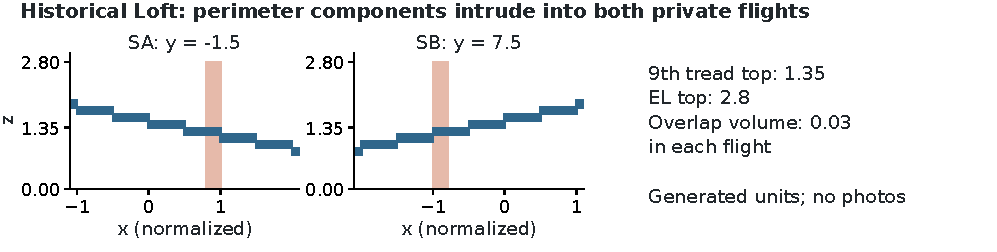
\includegraphics[width=.98\linewidth]{figures/casebook/I01_loft_wall_two_stairs.pdf}
\caption{Historical Loft geometry: the same declared perimeter has components
crossing both private flights. The panels use original normalized coordinates.}
\label{fig:I1-loft}
\end{figure}

\subsection{I2: a Farnsworth endpoint misses its declared upper terrace}
\label{app:I2}

\textbf{Evidence.}
The historical eight-configuration matrix evaluated Farnsworth House using
three measured-drawing pages. GPT-5.6 Luna answered its fixed geometric
questions correctly in B0, but its independent B1 world failed NF05 under
instrument 2.0.0.

\textbf{Output and computation.}
The generated upper terrace occupies $x\in[0,22]$ ft. The upper-flight endpoint
is $(31,-0.05,2.333\ldots)$ ft, and its landing is also near $x=31$.
Although endpoint and terrace-floor elevations agree, the endpoint lies
outside the terrace footprint. The saved proof reports that the upper endpoint
is not on its room floor; the lower endpoint passes that check.

\textbf{Interpretation and reproduction.}
This is a determinate geometric connection failure, rather than malformed
JSON. A connection label and an endpoint height do not establish incidence.
I2 retains the original endpoint, terrace, landing, and NF05 proof. The
historical result is not substituted into the current N2 table.

\begin{figure}[htbp]
\centering
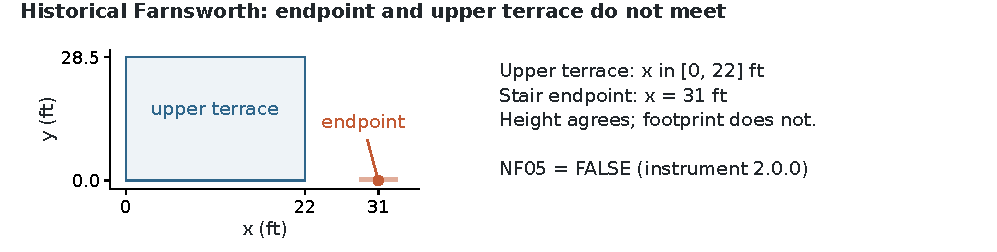
\includegraphics[width=.98\linewidth]{figures/casebook/I02_farnsworth_endpoint.pdf}
\caption{The generated endpoint and landing are laterally outside the
declared upper terrace. Equal height does not provide the missing contact.}
\label{fig:I2-endpoint}
\end{figure}

\subsection{I3: queried identity and unregistered material are different scopes}
\label{app:I3}

\textbf{Evidence.}
For Idaho City Schoolhouse, the N2 GPT-5.6 Luna B world satisfies all eight
fixed queries and passes registered geometry. Q08 correctly maps two
observations to \texttt{STAIR\_INTERNAL}. The exterior stair, not this
internal stair's material, belongs to the registered geometric obligations.

\textbf{Output and computation.}
The internal run rises from $(45,11,0)$ to $(45,17,10)$ ft in sixteen steps.
The uncut upper slab occupies $z\in[8,10]$ ft. The frozen material proof
identifies three tread surfaces at $8.125$, $8.750$, and $9.375$ ft,
covered across their full three-foot width.

\textbf{Interpretation and reproduction.}
Q08 checks the internal stair's identity, and that assignment is correct.
Its material is outside registered geometric scope but
inside all-declared scope. Extract I3 retains that scope list, Q08, and the
slab/run coordinates. Duplicate proof rows describe one physical conflict.

\begin{figure}[htbp]
\centering
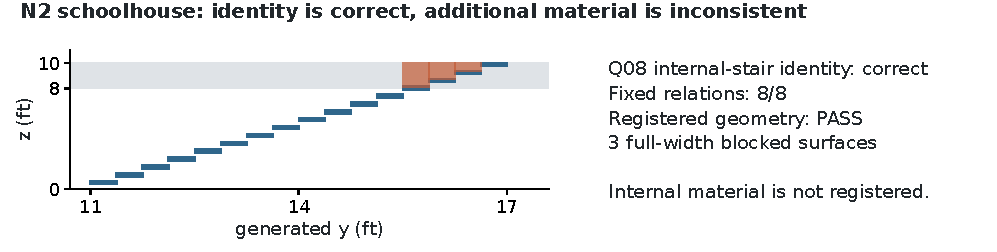
\includegraphics[width=.98\linewidth]{figures/casebook/I03_c03_registered_vs_material.pdf}
\caption{Identity is correct in Q08, while the internal-stair material is
inconsistent. Registered exterior-stair geometry remains a separate check.}
\label{fig:I3-scope}
\end{figure}

\subsection{I4: Lovell landing height is present but geometrically inconsistent}
\label{app:I4}

\textbf{Evidence.}
The CS1 Qwen model \texttt{qwen3.8-max-0902} produced a contract-valid
independent world for Lovell House. The fixed reference for Q09 requires
a staircase connection; evaluator 2.2.1 returns \texttt{UNKNOWN}.

\textbf{Output and computation.}
Landing \texttt{ld\_T03m} explicitly declares
\texttt{floor\_z=5.29} ft. Its box spans $z\in[5.29,5.79]$ ft.
The lower run also ends at $z=5.29$ ft. The floor field therefore agrees
with the material bottom rather than the supporting top. The saved reader
reports that the landing material and declared floor level are inconsistent.

\textbf{Interpretation and reproduction.}
This is not simply a missing-field error, nor evidence of a missing
visual detection. The available artifact localizes the failure to executable
support semantics. I4 compares the original landing box, floor field, run
endpoint, and Q09 proof without inserting a new platform or modifying a
height. Its unresolved readout remains distinct from a determinate false
connection.

\begin{figure}[htbp]
\centering
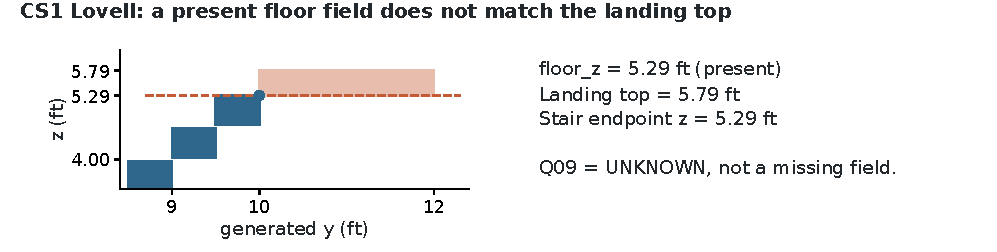
\includegraphics[width=.98\linewidth]{figures/casebook/I04_qwen_lovell_landing.pdf}
\caption{Lovell's generated landing floor is at its box bottom, 0.5 ft below
the material top. The field exists; its geometric meaning is inconsistent.}
\label{fig:I4-landing}
\end{figure}

\subsection{I5: a zero-thickness Astra landing violates the box contract}
\label{app:I5}

\textbf{Evidence.}
In the historical Farnsworth B1 artifact from GPT-6 Astra, NF05 is
\texttt{NOT\_EVALUABLE} under instrument 2.0.0. The JSON parses, but required
landing geometry is not executable.

\textbf{Output and computation.}
The upper-flight top interface has a positive rectangular footprint.
Both its minimum and maximum $z$ equal $2.333\ldots$ ft.
Consequently its box height is zero. The declared primitive requires
finite, strictly positive extent on all three axes; the compiler records
\texttt{INVALID\_GEOMETRY}.

\textbf{Interpretation and reproduction.}
A mathematical surface can be a reasonable intended interface while
violating this particular occupied-box representation. This observation
does not prove that the physical connection is impossible or that the
model reversed the building's levels. I5 preserves the zero-height box
and historical refusal. We do not thicken the interface or award a
counterfactual score.

\begin{figure}[htbp]
\centering
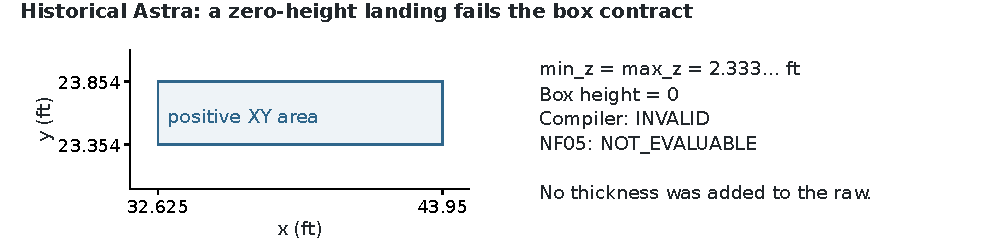
\includegraphics[width=.98\linewidth]{figures/casebook/I05_astra_zero_height.pdf}
\caption{Positive plan area does not satisfy a positive-volume box contract:
the original landing has exactly zero height.}
\label{fig:I5-contract}
\end{figure}

\subsection{I6: equivalent slab material triggers a different alarm}
\label{app:I6}

\textbf{Evidence.}
An existing diagnostic starts from Qwen's N2 Octagon House B output.
It changes only the slab's box encoding and retains the same opening.
This is a deterministic instrument diagnostic, not a new model response.

\textbf{Output and computation.}
Encoding one uses four pre-cut slab boxes; encoding two uses their envelope
with the same opening subtracted. The saved mutual-containment and difference
checks establish equal final material, with volume $155.489115$ ft$^3$.
Nevertheless, 2.2.1 reports one \texttt{DETACHED\_OPENING} row for the first
encoding and none for the second.

\textbf{Interpretation and reproduction.}
This establishes an encoding-sensitive instrument limitation, not a
physical obstruction. Four other violations remain unchanged; both full
verdicts are still \texttt{VIOLATION}. Fixed readouts and registered
geometry do not change. I6 retains both encodings, the unchanged void, and
the original equivalence proof; the diagnostic does not replace a primary
score.

\begin{figure}[htbp]
\centering
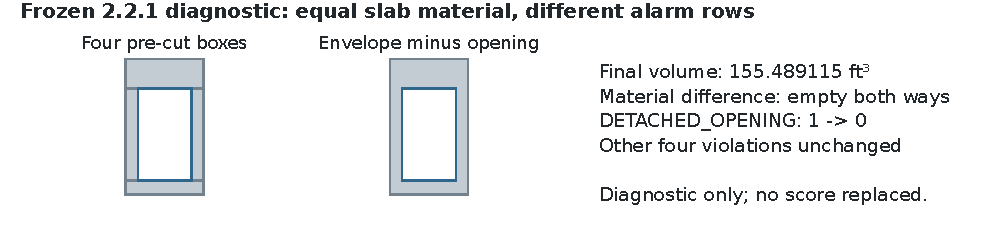
\includegraphics[width=.98\linewidth]{figures/casebook/I06_equivalent_slab_alarm.pdf}
\caption{Equal final slab material has different detached-opening alarm
counts. The diagnostic removes one alarm, not all remaining violations.}
\label{fig:I6-instrument}
\end{figure}

\subsection{I7: a genuine positive declared fragment}
\label{app:I7}

\textbf{Evidence.}
The N2 GPT-6.1 Terra A output for San Xavier del Bac provides a positive
control from the same frozen main-results collection, not a hand-built
reference or an \texttt{UNKNOWN} result.

\textbf{Output and computation.}
The world contains lower and upper tower spaces, a nave fragment, walls,
door and window openings, a font, and an upper support slab. All six fixed
relations are correct, all five target roles are present, registered
geometry passes, and verification is
\texttt{PASS\_DECLARED\_FRAGMENT}. The saved joint fragment-success flag is
true. The figure shows its actual hypothetical coordinate completion.

\textbf{Interpretation and reproduction.}
The benchmark admits successful worlds; failures are not required by its
definition. This positive applies to the bounded declaration and implemented
checks. It does not certify unseen parts of the mission or human navigation.
I7 reproduces the unchanged entity geometry, coverage record, query values,
and full-declaration verdict. The geometry and score are retained rather
than simplified into a synthetic ideal example.

\begin{figure}[htbp]
\centering
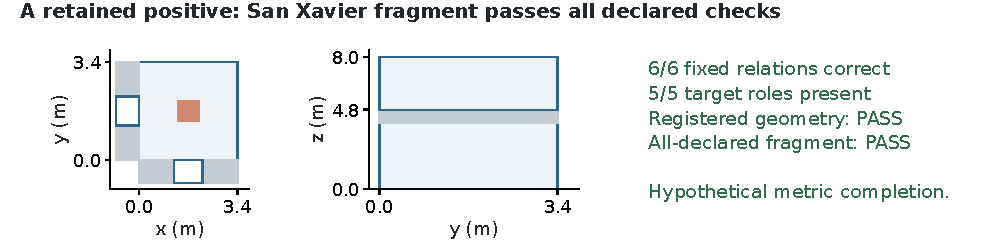
\includegraphics[width=.98\linewidth]{figures/casebook/I07_true_fragment_pass.pdf}
\caption{Tower detail of a real positive: six correct fixed relations, all five target
roles, and both registered and all-declared fragment checks pass.}
\label{fig:I7-positive}
\end{figure}

The supplied casebook verification script recomputes the numerical witnesses using only the Python standard library. Historical scores and unsupported semantic checks remain \texttt{NOT\_RECOMPUTED}.
